\def\year{2019}\relax
\documentclass[letterpaper]{article}
\usepackage{aaai19}
\usepackage{times}
\usepackage{helvet}
\usepackage{courier}
\usepackage{url}
\usepackage{graphicx}
\usepackage{tabularx} % For improving the table
\usepackage{array}
\usepackage{tikz}
\usepackage{multirow}
\usepackage{pifont}
\usepackage{float}
\def\tabularxcolumn#1{m{#1}}
\newcolumntype{Y}{>{\centering\arraybackslash}X}
\frenchspacing
\setlength{\pdfpagewidth}{8.5in}
\setlength{\pdfpageheight}{11in}
%PDF Info Is Required:
%\pdfinfo{
%/Title (Title will go here)
%/Author (Zach Wilkerson, Keisuke Ohtani)}
\setcounter{secnumdepth}{0}  
\begin{document}
\title{Using Gradient Boosting, Pre-processing, and Parameterization to Estimate Housing Prices in CSC396}
\author{Zach Wilkerson, Keisuke Ohtani\\
DePauw University\\
Greencastle, IN 46135, U.S.A.\\
\{zwilkerson\_2020, keisukeohtani\_2019\}@depauw.edu\\
}
\maketitle
\begin{abstract}
In the housing market, a multitude of factors influence final selling prices, and it is frequently very challenging to accurately quantify the influence of these factors.  Our work sought to address this problem by creating a Scikit-learn gradient boosting regression ensemble and by exploring pre-processing and parameterization techniques to refine predictive models based on provided feature data.  We designed an algorithm capable of achieving a maximum R-squared value of 0.9728 using 10-fold cross-validation on the training data set, thus presenting a promising approach to creating a reliable predictor.
\end{abstract} 

\section{Introduction}

One reason that machine learning algorithms exist is for the modeling of complex problems.  Keeping with this rationale, our work encompasses a project for a Data Mining course at DePauw University.  The project itself is based on the Kaggle competition, ``House Prices: Advanced Regression Techniques," in which competitors are given a data set containing properties of recently-sold houses in Ames, IA, along with their respective selling prices (for detailed information, see Data Description section).  From these data, we created a regressor model using various pre-processing methods and machine learning algorithm parameterization techniques.

\section{Data Description}

The provided data set contains 79 features categories pertaining to different properties of houses (e.g., basement finish, lot size, garage quality, distance to nearest railroad, pool condition, etc.) and one output category for the selling price of the house; each row corresponds to a single house.  Individual rows may not include values for each feature; in the raw data set, these absent values appear as ``NA."  Sometimes these missing values appear by coincidence, but in some cases (e.g., signifying the absence of a basement for the ``basement condition" feature) they are significant.

Data features present a mixture of numerical (e.g., date the house was sold) and nominal (e.g., basement condition) data.  Furthermore, nominal data values fall into several broad categories, such as ranked (e.g., basement condition) or cost-dependent (e.g., masonry veneer type).  Other nominal data values (e.g., MS zoning) have no obvious numeric analog.  By contrast, numeric data represent either discrete (e.g., MS. Subclass) or continuous (e.g., year built) values.  Our work does not focus significantly on this numeric distinction, but it is possible that feature engineering discriminating between ranges/segments of continuous values could improve upon the results described below.

\section{Experimentation}

Broadly, we sought to maximize the R-squared score of a regression model trained on the provided data set.  More specifically, we employed a variety of pre-processing and parameterization techniques to refine our model.  While we briefly explored other methods such as alternate learning algorithms, our primary focus was on pre-processing techniques, supported by experimental parameterization of a suggested gradient boosting regression ensemble.

\subsection{Pre-processing}

We applied pre-processing techniques in two primary stages to the regressor: preparation and optimization.  The preparation stage represents the programming required to achieve the first working model, as well as basic improvements (and subsequent experimentation) on this initial strategy, such as normalization and standardization.  The optimization stage encompasses conceptual improvements that use the preparation-stage code as a springboard to maximize the R-squared value of the resulting model.

\subsubsection{Preparation}

In order to create the first model, all ``NA" values needed to be processed, and all features had to be converted to numeric values.  Nominal-to-numeric value translation was accomplished using the LabelEncoder transform function, which assigns a numeric index to each instance of a unique nominal value.  We favored this approach over one-hot encoding (which generates an unnecessary amount of features) and binary encoding (which might foster coincidental relationships between features in future tests).  This approach by itself generated an error when processing ``NA" values within otherwise numeric feature groups, and even when successful it treated ``NA" as its own value (which was sometimes incorrect given the nature of the data set outlined in the Data Description section).  In response, a function was created to discriminate between these ``insignificant NA values" and the ``significant NA values."  This function identified features for which a value of ``NA" was significant and then translated ``NA" into ``NoValue," which would then be translated by the encoder function.  ``NA" values corresponding to data gaps were filled using the mode of values in the feature category across all rows.

Following these steps, we implemented functions for all features to decrease bias from large feature values (e.g., year sold).  Our normalization function followed the formula ${x_{new} = \frac{x - x_{min}}{x_{max} - x_{min}}}$, and our standardization function was denoted by ${x_{new} = \frac{x - \mu_{x}}{\sigma_{x}}}$.  In experimental testing, normalization was found to be slightly more effective than standardization for this problem (see Experimentation: Results section for details), and so normalization is an assumed part of subsequent pre-processing strategies.

\subsubsection{Optimization}

The greatest weakness of the initial nominal-to-numeric encoder was that the resultant integer-based indices were essentially random, providing little information to the machine learning algorithm besides a simple analog.  It is additionally possible that these indices suggested order within feature groups where no order was present.  To address this issue, we developed more ``intelligent" methods of pre-normalization nominal value encoding, based on the categories of nominal values described previously.  For nominal ranked values, a simple analog was created equating 1 with the best/greatest value (e.g., ``excellent" in quality evaluations) down to equating 0 with the worst/least value (e.g., ``poor" or ``NoValue").  For nominal cost-dependent values, each nominal value was encoded to an estimated per-unit analog found online (e.g., price for masonry veneer type, referencing Angie's List).

However, our greatest R-squared improvement resulted from our encoding strategy as applied to nominal data with no apparent pattern among values (see Experimentation: Results section for details).  These values were encoded using the median sale price (output value) among all rows containing the same value.  For example, the ``Street" feature has ``Gravel" and ``Paved" values. We separated houses into groups based on the value (either ``Gravel" or ``Paved") and calculated the median selling price for each group. Then, values with ``Gravel" were replaced with the median of all ``Gravel" selling prices, and values with "Paved" were replaced with the median of all "Paved" selling prices, greatly improving the R-squared score as a result.

\begin{table}
\begin{center}
\begin{tabularx}{\columnwidth}{>{\hsize=0.1\hsize}X >{\hsize=1.25\hsize}Y} 
\hline
\multicolumn{1}{c}{\textbf{Value}} & \multicolumn{1}{c}{\textbf{Description}} \\ \hline
20 & 1-story 1946 newer all styles \\
30 & 1-story 1945 older \\
40 & 1-story w/finished attic all ages \\
45 & 1-1/2 story - unfinished all ages \\
50 & 1-1/2 story finished all ages\\
60 & 2-story 1946 newer\\
70 & 2-story 1945 older\\
75 & 2-1/2 story all ages\\
80 & split OR multi-level\\
85 & split foyer\\
90 & duplex - all styles and ages\\
120 & 1-story PUD - 1946 newer\\
150 & 1-1/2 story PUD - all ages\\
160 & 2-story PUD - 1946 newer\\
180 & PUD - multilevel - incl split lev/foyer\\
190 & 2 family conversion - all styles and ages\\
\end{tabularx}
\end{center}
\caption{MSSubClass identifies the type of dwelling involved in the sale (PUD = planned unit development).}
\label{tab:msSubclass}
\end{table}

\begin{figure*}
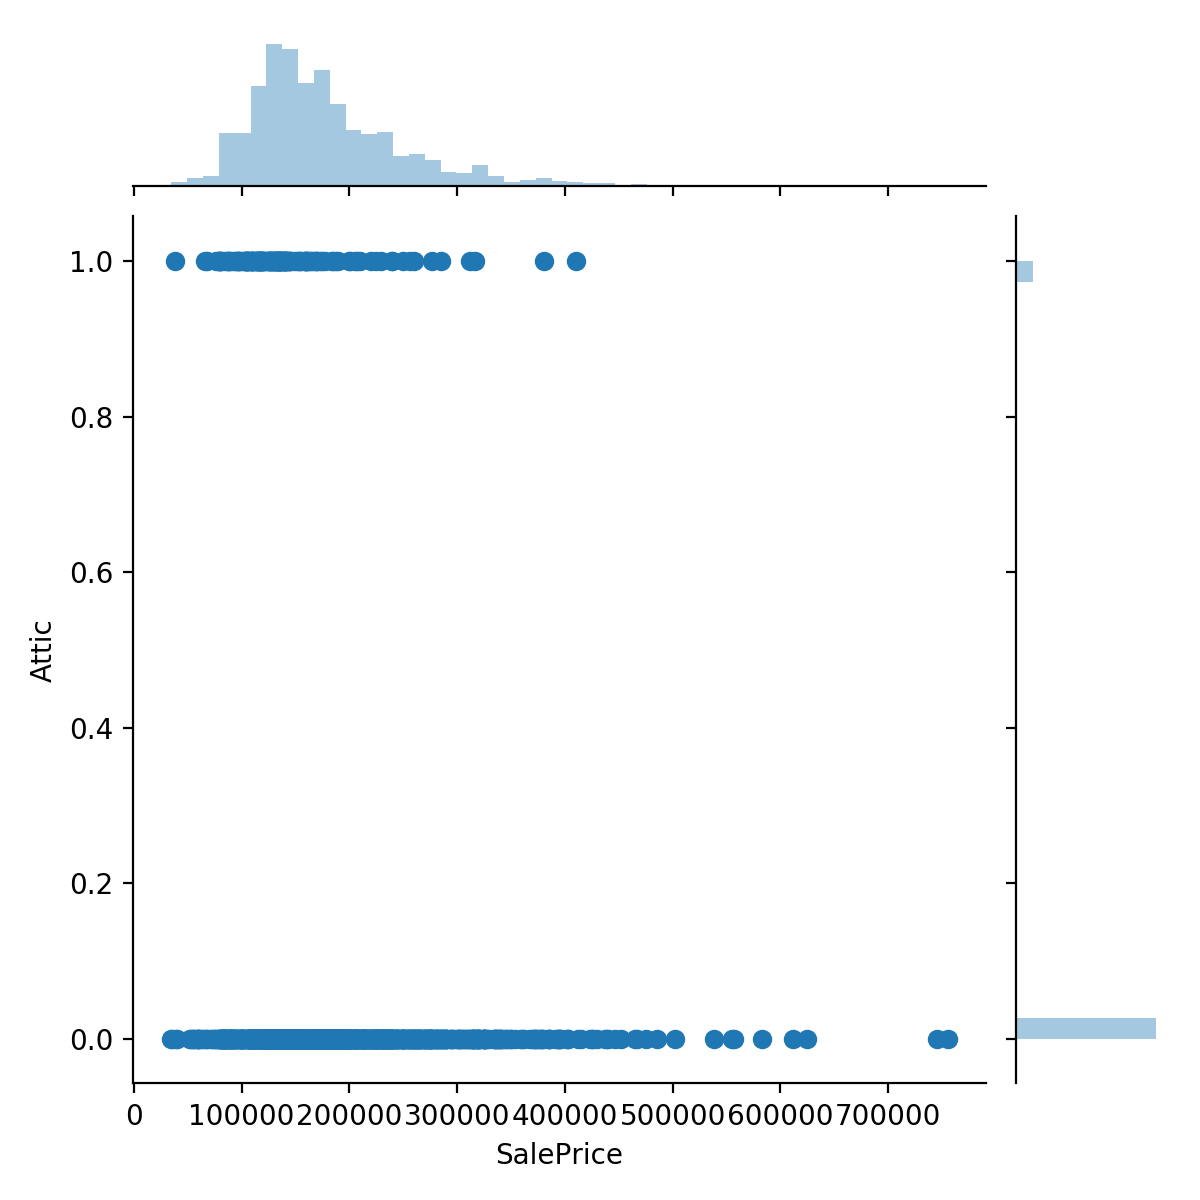
\includegraphics[width=.33\textwidth]{Figure_1.png}
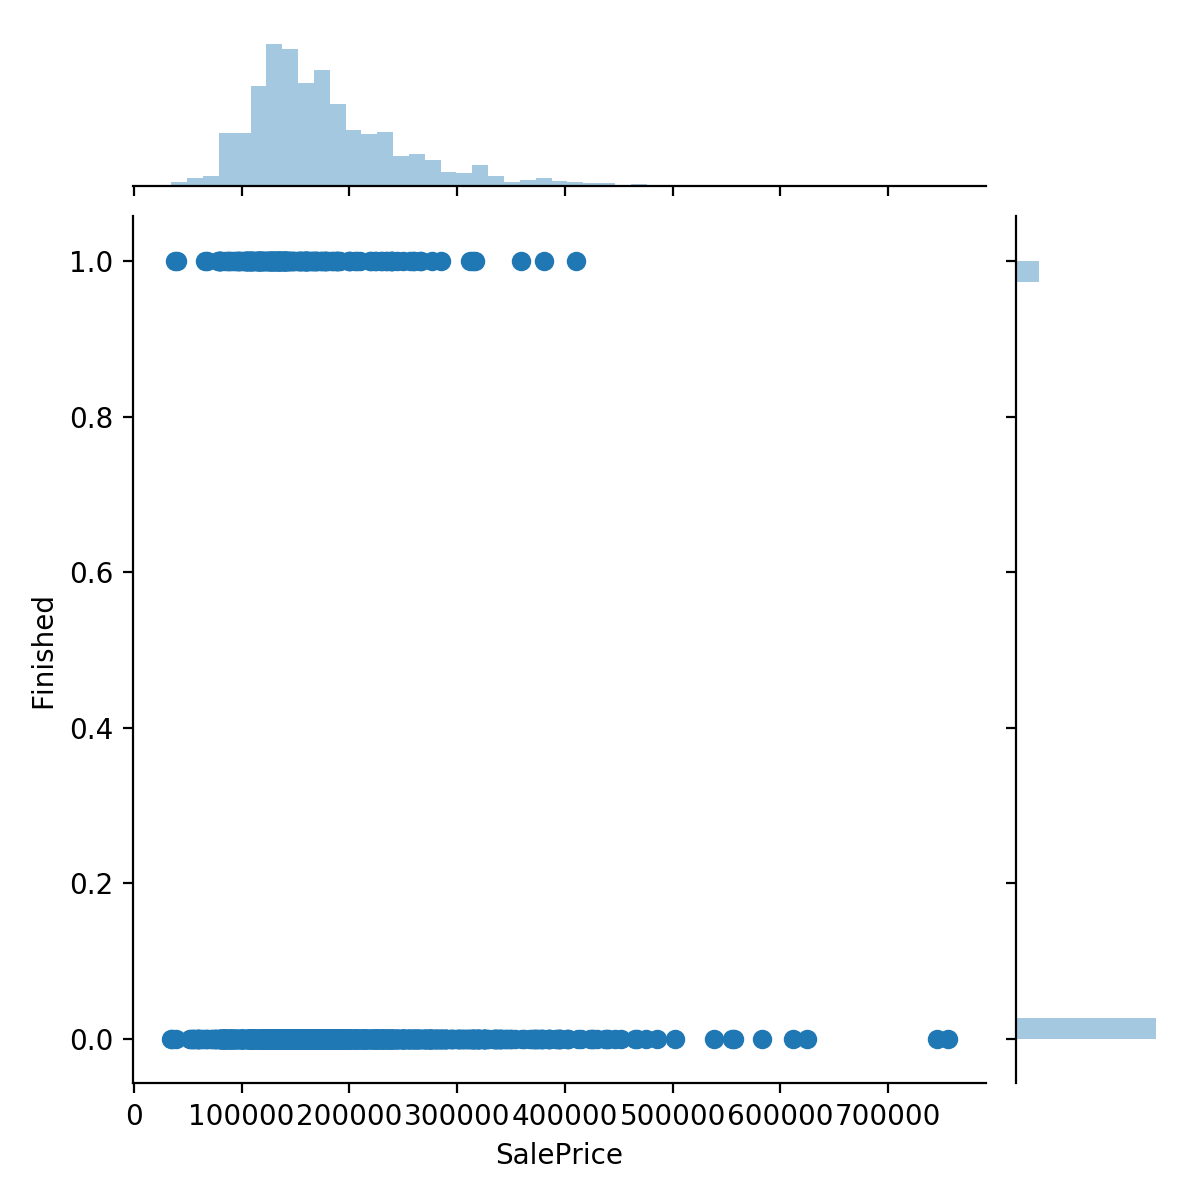
\includegraphics[width=.33\textwidth]{Figure_2.png}
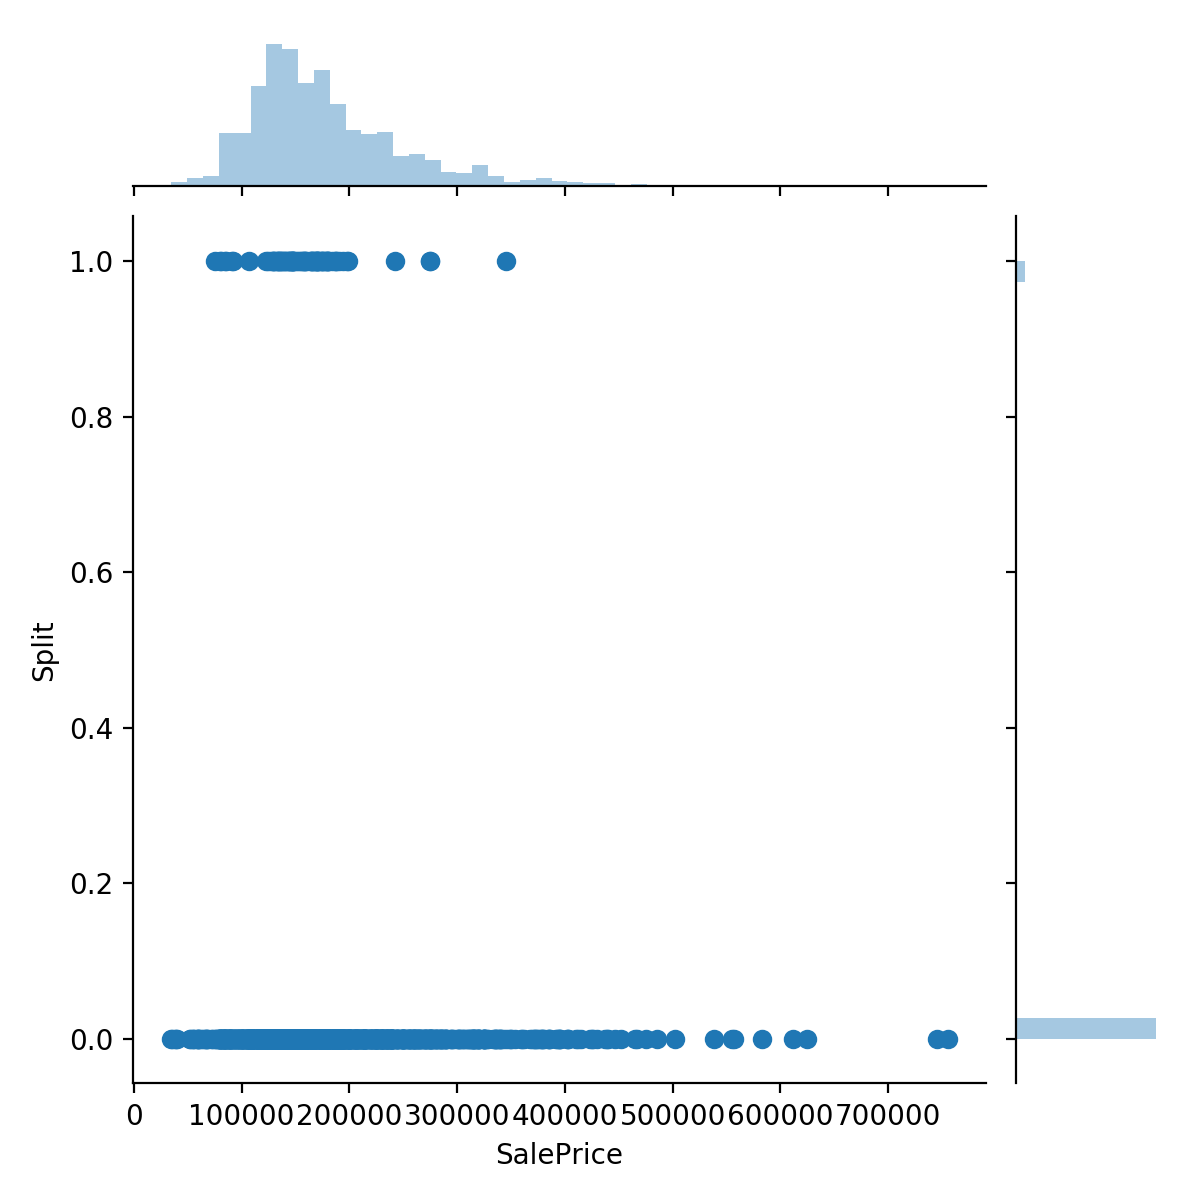
\includegraphics[width=.33\textwidth]{Figure_3.png}
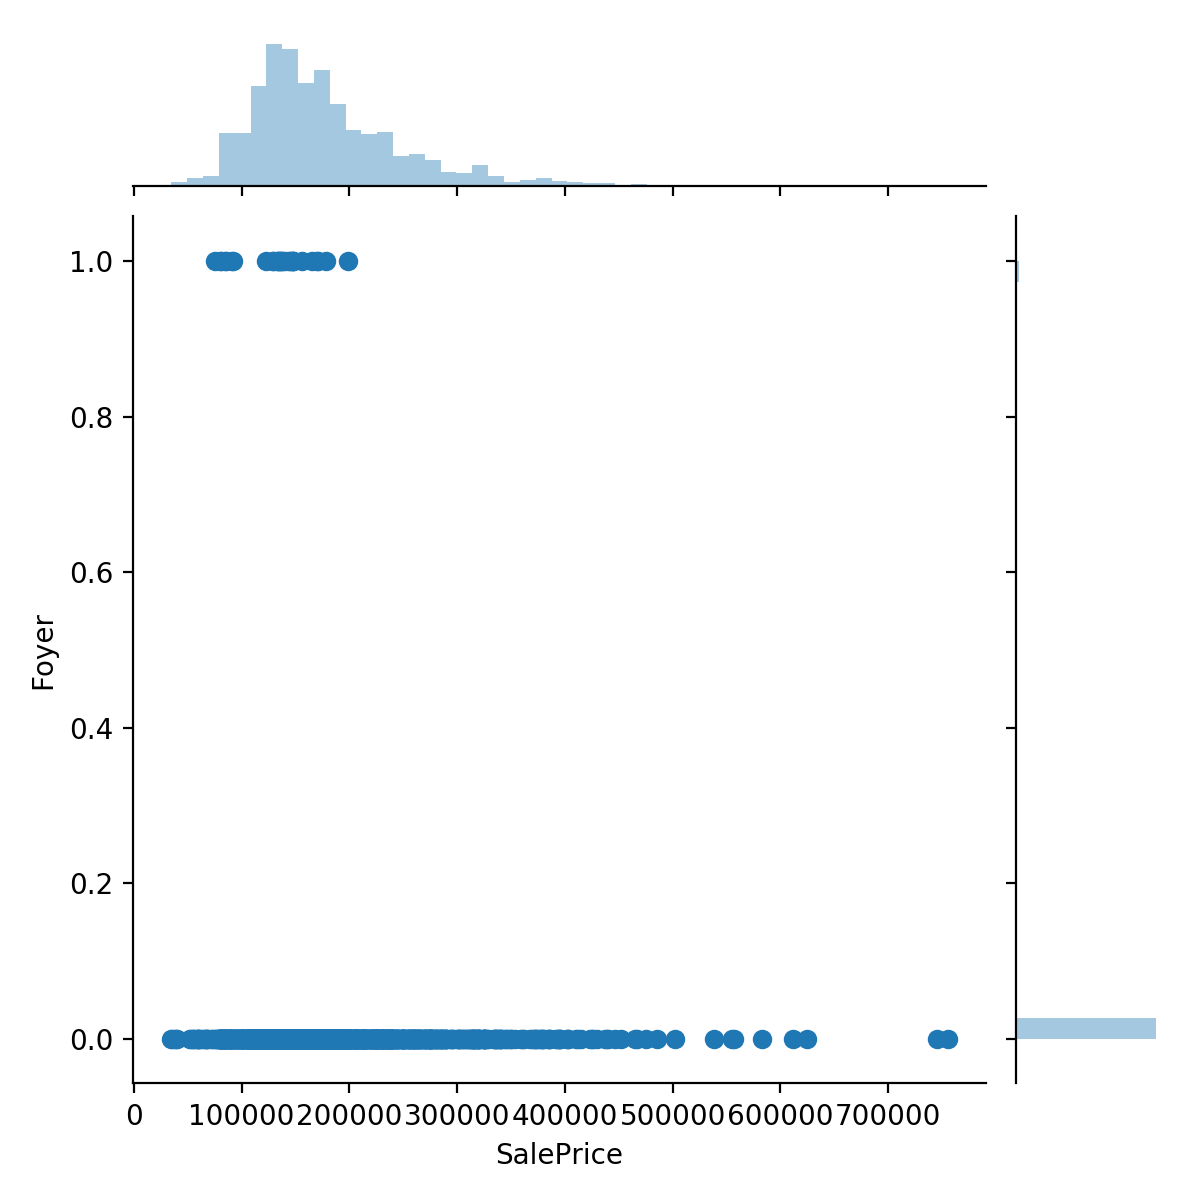
\includegraphics[width=.33\textwidth]{Figure_4.png}
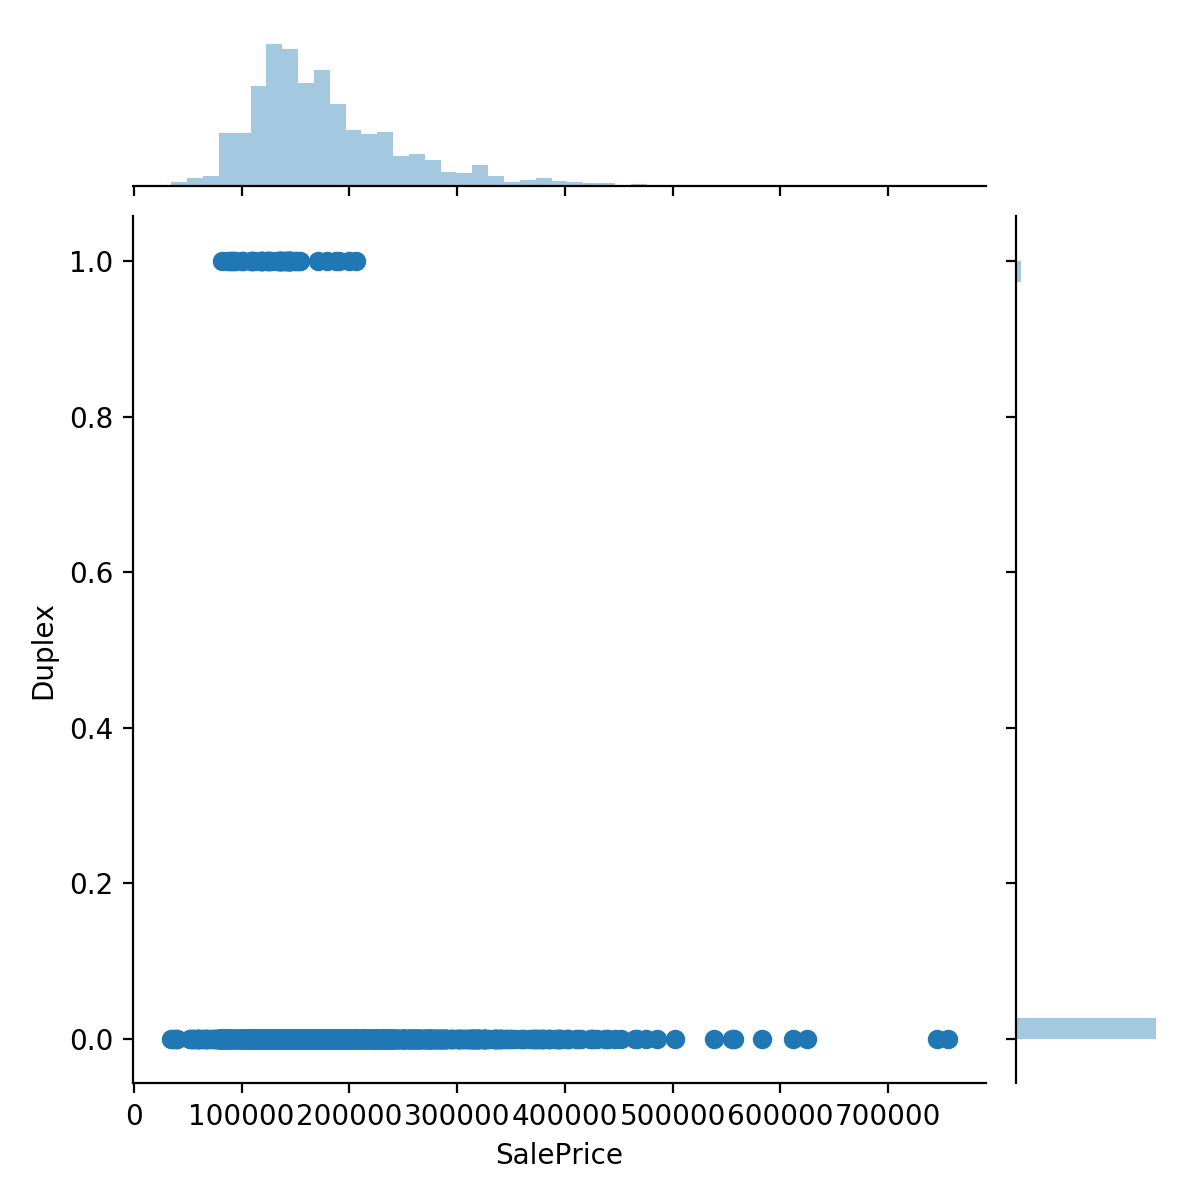
\includegraphics[width=.33\textwidth]{Figure_5.png}
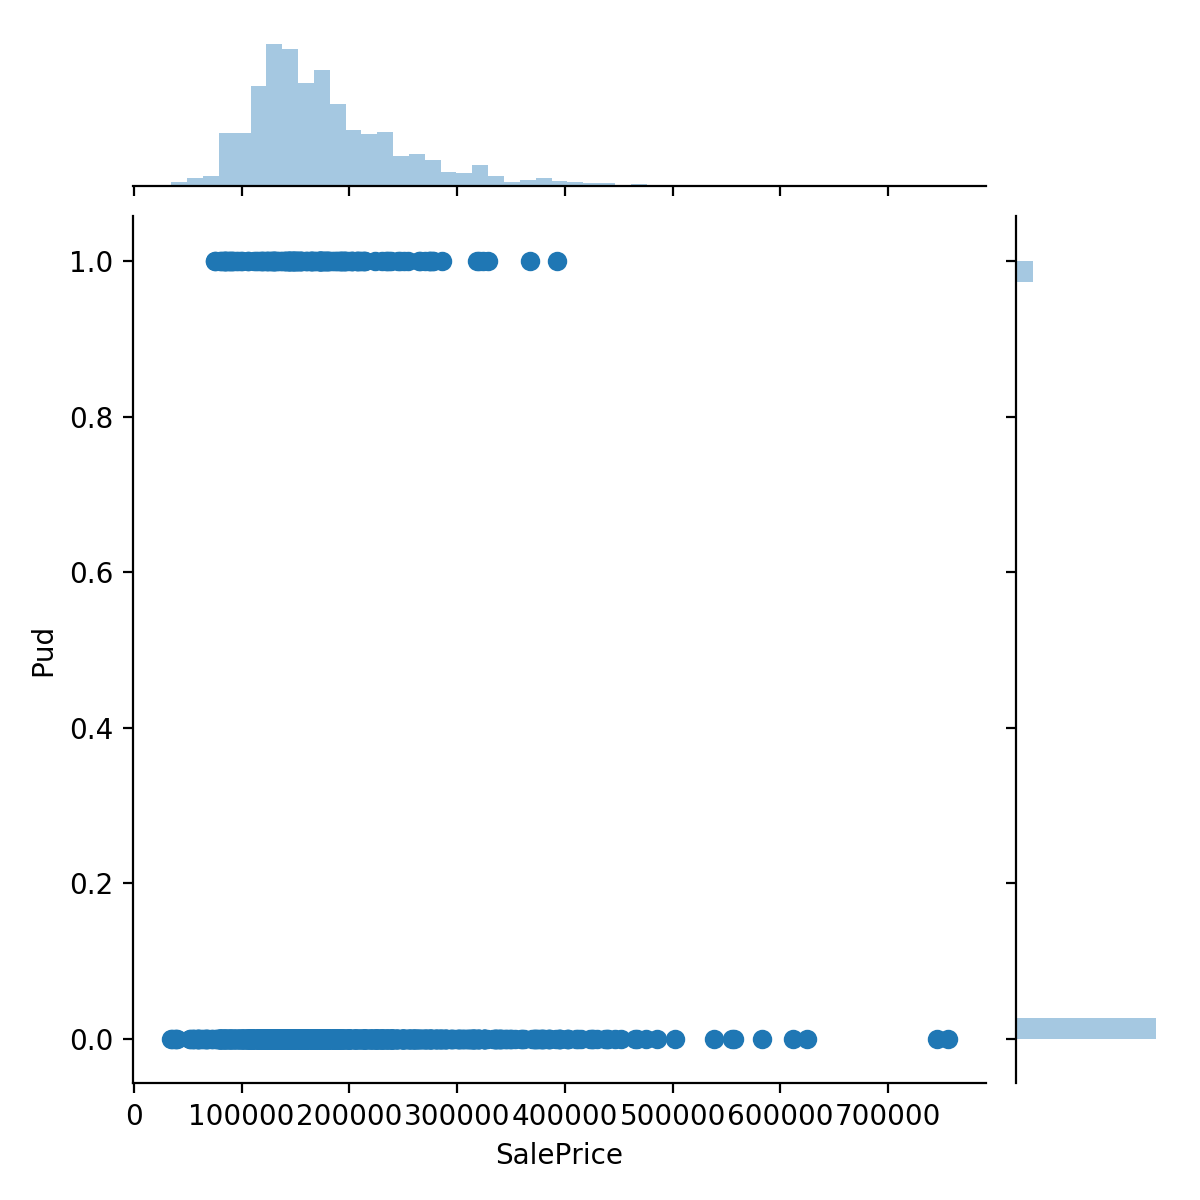
\includegraphics[width=.33\textwidth]{Figure_6.png}
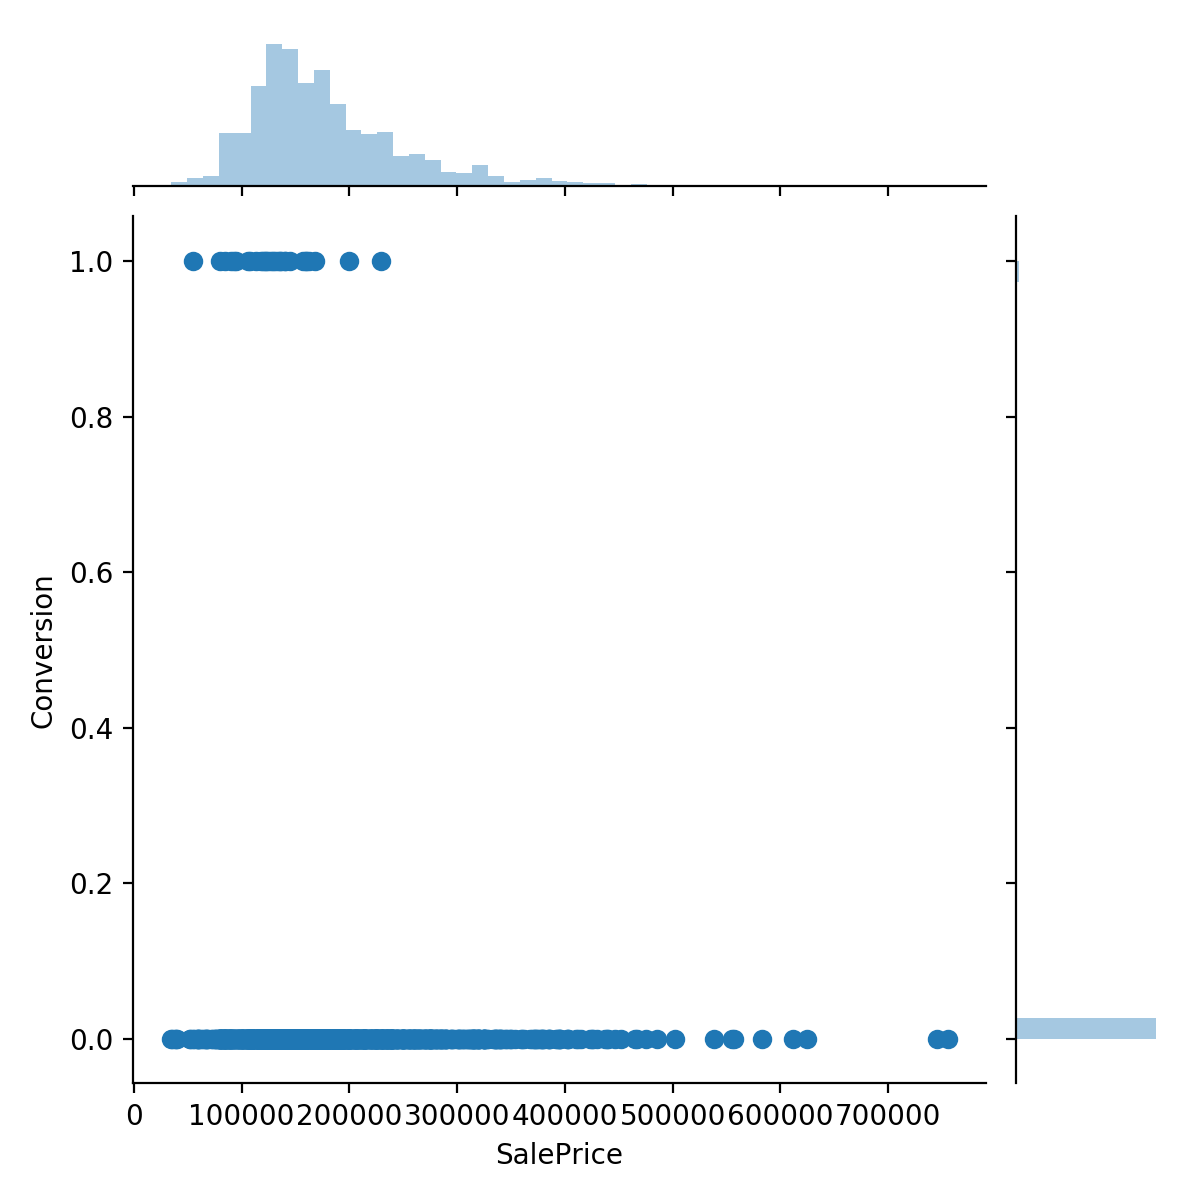
\includegraphics[width=.33\textwidth]{Figure_7.png}
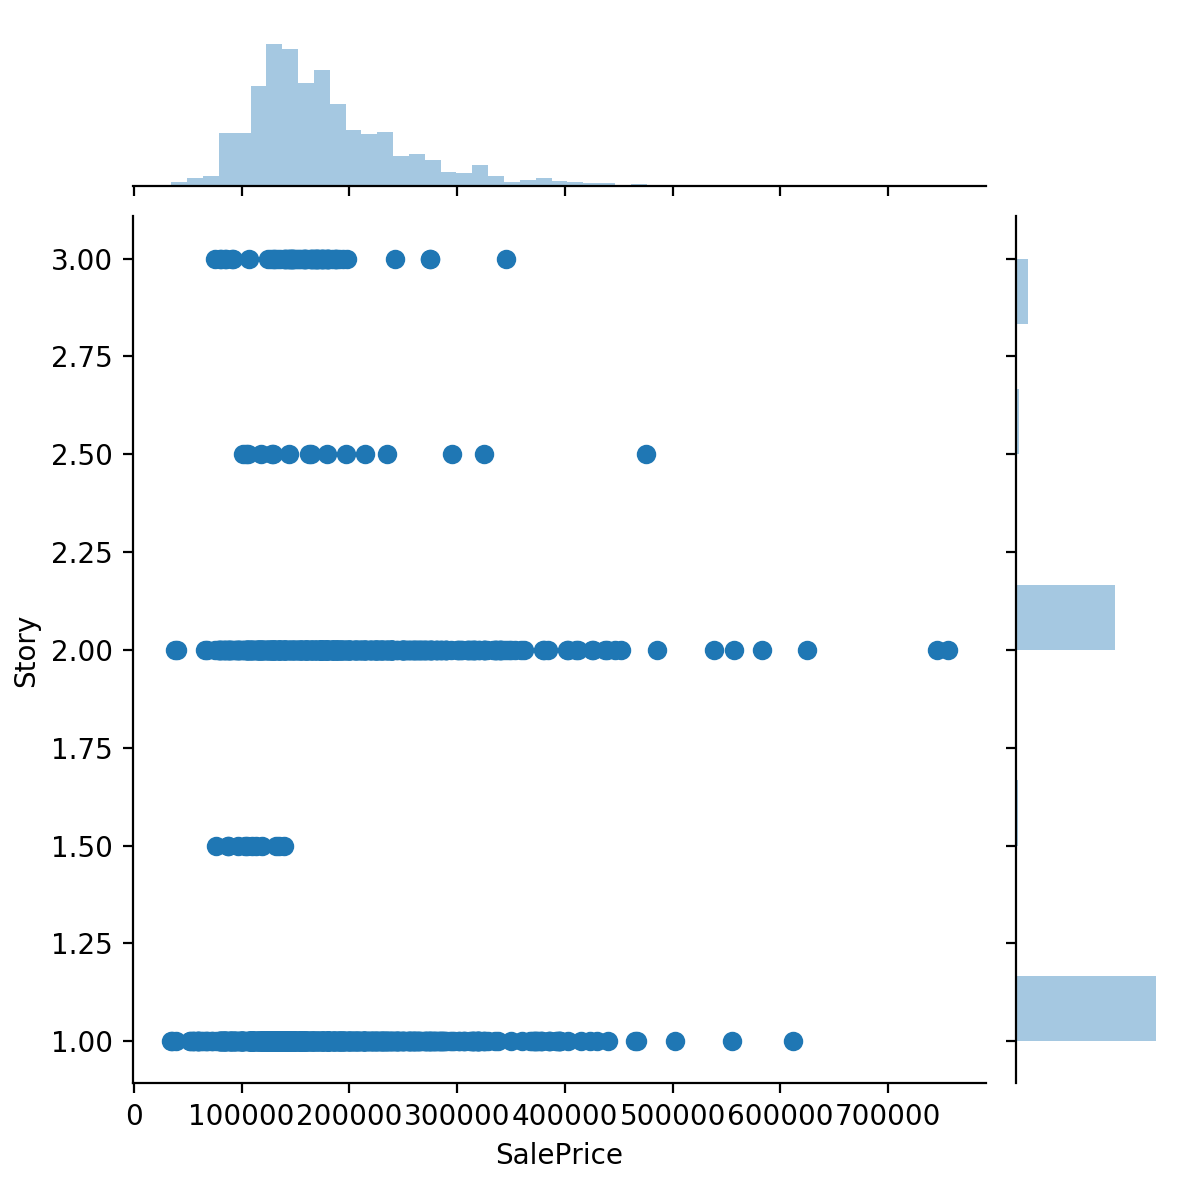
\includegraphics[width=.33\textwidth]{Figure_8.png}
\caption{Each feature and selling price joint plot.}
\label{fig:msDivisions}
\end{figure*}

\begin{figure}
\begin{center}
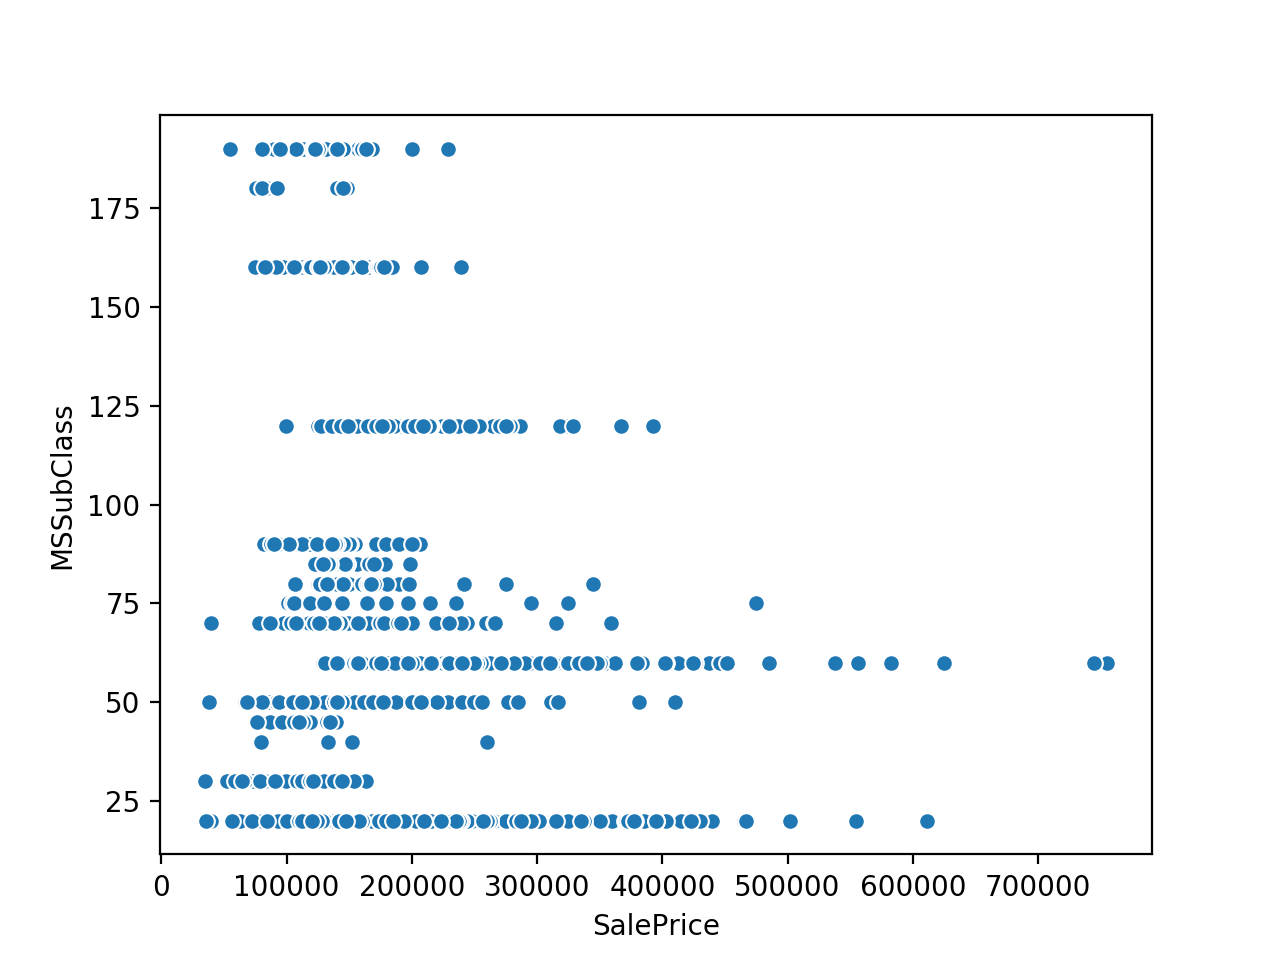
\includegraphics[width=\columnwidth]{MSSubClassJointplot.png}
\caption{MSSubClass feature distribution versus selling price.}
\label{fig:msWhole}
\end{center}
\end{figure}

\subsubsection{Additional Notes}

Following the optimization stage, we experimented with editing some of the numerical data entries as well.  Specifically, we tested whether representing features relating to a year as an age instead would improve the R-squared score.  Of two numeric categories, this was true for one (``Year Built").  Any R-squared score improvements resulting from parameterization (described in the following section) follow this improvement.

Upon deeper analysis of the data description documentation, we noticed that ``MSSubClass" column appeared to combine multiple features (Table \ref{tab:msSubclass}). However, when we experimented with splitting the ``MSSubClass" into ``Attic", ``Finished", ``Split", ``Foyer", ``Duplex", ``Pud", ``Conversion", and ``Story" features, the R-squared score was essentially unaffected (it actually decreased slightly). We concluded that even though this breakdown appeared logical, it did not provide strong metrics with which to make predictions (Figure \ref{fig:msDivisions}). Thus, we observed no real improvement over the default feature classification (Figure \ref{fig:msWhole}).

Lastly, we experimented with the possibility of removing features, as we had only explored hypotheses that improved how we looked at the features as a whole (and not what subset of features might prove most useful).  While the numeric results are presented in Table \ref{tab:remove_feature}, we generally found that removing certain individual features would improve model performance.  However, we observed unexpected relationships between features when actually removing them (particularly removing multiple at a time, see Experimentation: Results section for details).

\subsection{Algorithms and Parameterization}

Our model was a Scikit-learn gradient boosting regression ensemble, using a random\_state parameter of 1 to minimize bias in model generation.  Broadly, this model makes a general prediction, then aggregates a given amount of predictors, each one modifying the previous aggregate prediction (usually by a decreasing absolute amount).  Once a certain threshold is reached (e.g., the number of predictors aggregated), the process halts and returns the net prediction.

We experimented with parameters controlling the number of predictors aggregated and the learning rate of the algorithm (i.e., how drastically each predictor changes the prediction).  We found that optimizing either parameter further increased the R-squared value, but that using these optimized values simultaneously did not result in as great an increase in accuracy.  As a result, our final model incorporates only the optimized number of estimators parameterization.

In addition to investigating parameters for the gradient boosting regression ensemble, we briefly explored linear regression as an alternative model.  Linear regression uses gradient descent to find a regression estimate for a given n-dimensional space (a line for 2-D, a plane for 3-D, and a hyperplane for higher-dimensional spaces).  The results from these tests suggested that linear regression was not a suitable model for our data set, or at least that a complete do-over of all pre-processing steps would be required to correctly prepare the data.

\begin{table}
\begin{center}
\begin{tabularx}{\columnwidth}{>{\hsize=1\hsize}X >{\hsize=0.5\hsize}Y} 
\hline
\multicolumn{1}{c}{\textbf{Feature Removed}} & \multicolumn{1}{c}{\textbf{R-squared Value}} \\ \hline
Building Type & 0.9736 \\
Year Built & 0.9735 \\
Land Slope & 0.9733 \\
Half Bath & 0.9731 \\
Basement Finish Type 2 & 0.9730 \\
... & ... \\
Nothing Removed & 0.9728 \\
... & ... \\
Functionality & 0.9710 \\
Street & 0.9705 \\
Second Floor Square Footage & 0.9733 \\
Ground Floor Living Area & 0.9612 \\
Lot Area & 0.9603 \\
\end{tabularx}
\end{center}
\caption{Selected resulting R-squared values for removing a single feature.}
\label{tab:remove_feature}
\end{table}

\subsection{Results}

\begin{figure*}
\begin{center}
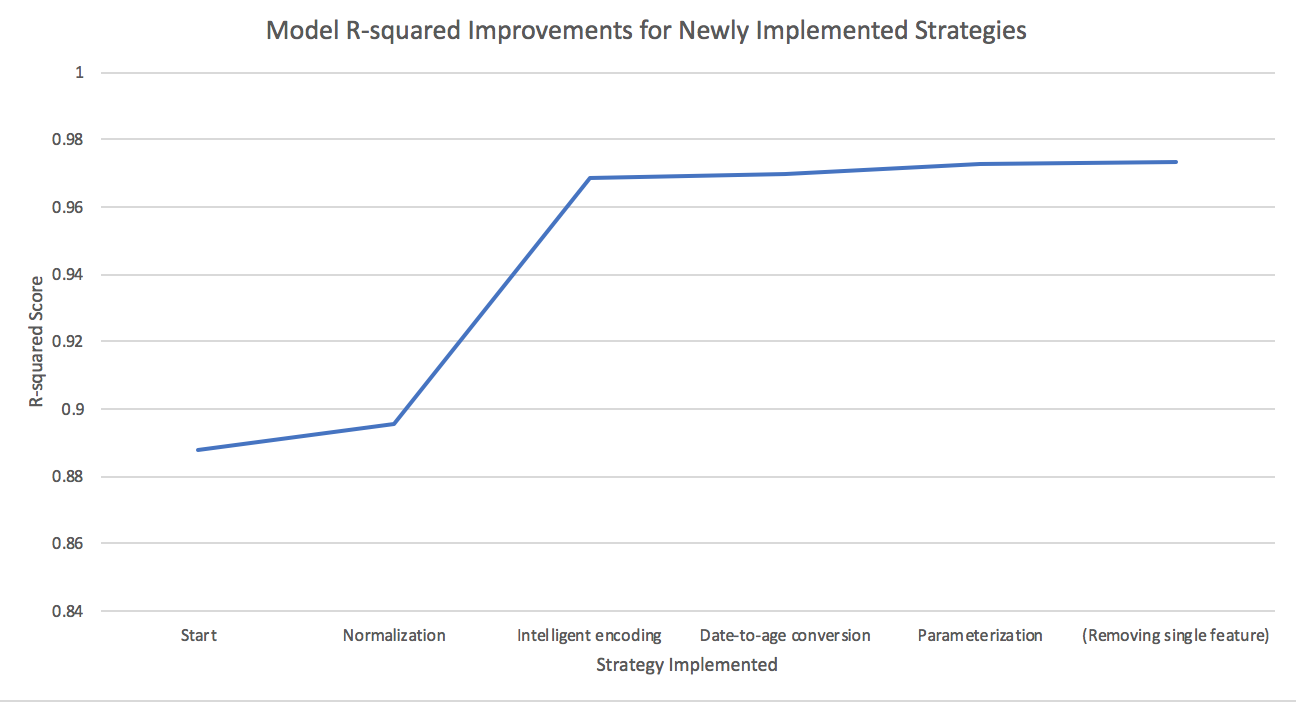
\includegraphics[width=\textwidth]{Figure.png}
\end{center}
\caption{Plot of model's R-squared score progression.}
\label{fig:results}
\end{figure*}

While our testing of different pre-processing and parameterization strategies resulted in surprisingly consistent data results, we truncate at four significant digits to afford a reasonable margin of error.  Overall, our highest achieved accuracy was 0.9728, with the potential of 0.9736 after removing one particular feature (Table \ref{tab:remove_feature}).

Our first successful test of the gradient boosting regression model (using only the LabelEncoder translation) yielded a mean R-squared value of approximately 0.8879 using 10-fold cross-validation.  After including normalization, this accuracy increased to 0.8958 (standardization afforded an increase to 0.8952).  Our use of intelligent encoding resulted in a jump to 0.9684, which was modestly improved to 0.9696 after implementing a date-to-age conversion for the ``Year Built" feature.  After optimizing the number of estimators algorithm parameter (to 800 from a default value of 100), we achieved our final consistent R-squared value of 0.9727 (Figure \ref{fig:results}).

Two final interesting results that we observed concern the removal of features and linear regression.  While Table \ref{tab:remove_feature} represents changes (including improvements) in accuracy resulting from removing any one feature, we observed that removing multiple at once frequently reduces any benefit and sometimes leads to a reduction of accuracy.  Regarding linear regression, we observed an extraordinarily high degree of error (so much so that we also investigated root mean squared error as well, achieving values exceeding ${10^{22}}$), again suggesting a significant divide between our pre-processed data and the algorithm itself.

\subsection{Analysis}

An R-squared value does not directly correlate with accuracy; rather it represents the ``narrowness" of the margin for error from the regression prediction.  Regardless, an R-squared value so close to 1 is very promising for our approach.  Additionally, the relatively drastic growth in the R-squared value as a result of implementing intelligent nominal-to-numeric encoding (especially the general encoding to median price) suggests that pre-processing strategies of this type are particularly effective for the gradient boosting regression algorithm.  This makes sense, given that it arguably was most instrumental in making the otherwise diverse data set more uniformly formatted.

In the realm of other interesting conclusions, the relative effectiveness of certain pre-processing and algorithm-level strategies is important to note.  In particular, normalization is slightly more effective than standardization; on the surface, this suggests that the data are somewhat randomly distributed, but that some discrepancies (possible feature relationships?) may persist.  The fact that the number of estimators seems more important than the learning rate is also significant.  We hypothesize that this is so given that increases in the number of estimators (resulting in more smaller adjustments) are effective for very small changes in data (which we were observing at the time of implementation), versus learning rate (frequently resulting in larger adjustments).  Lastly, the unusually large value for linear regression could suggest that the data do not lend themselves easily to linear regression (as opposed to polynomial regression, or another model).  However, with the possible existence of errors in the implementation of the linear regression model, further testing would be needed to confirm this conclusion.

Additional experimentation would also be required to provide greater understanding of the relationships between individual features highlighted in Table \ref{tab:remove_feature}.  For example, if we remove the feature yielding an optimal R-squared score and then recompute R-squared values for removing one of the remaining features, perhaps it would be possible to find an optimal set of features to remove from the data set for model creation.  Regardless, the results from Table \ref{tab:remove_feature} clearly support that feature removal (or feature engineering, possibly) could legitimately result in higher R-squared values then we have found so far.

\section{Conclusion and Acknowledgments}

While not perfect, our R-squared value of 0.9728 demonstrates a significant step toward a successful and reliable predictor model.  We hope in future work to focus on a subset of (at least) elimination of redundant/non-productive features, continued nominal data pre-processing experimentation, and model creation using other algorithms.  We thank Dr. Steve Bogaerts for his guidance and advice throughout this course and project, and we acknowledge Scikit-learn and Microsoft as two organizations whose products were integral to the successful conducting of this research.

\end{document}

